\documentclass{article}

\usepackage[utf8x]{inputenc}
\usepackage[english,russian]{babel}
\usepackage{cmap}
\usepackage{commath}
\usepackage{amsmath}
\usepackage{amsfonts}
\usepackage{mathtools}
\usepackage{amssymb}
\usepackage{parskip}
\usepackage{titling}
\usepackage{color}
\usepackage{hyperref}
\usepackage{cancel}
\usepackage{enumerate}
\usepackage{multicol}
\usepackage{graphicx}
\usepackage[font=small,labelfont=bf]{caption}
\usepackage[a4paper, left=2.5cm, right=1.5cm, top=2.5cm, bottom=2.5cm]{geometry}

\graphicspath{ {./images/} }
\setlength{\droptitle}{-3cm}
\hypersetup{ colorlinks=true, linktoc=all, linkcolor=blue }
\pagenumbering{arabic}

\begin{document}
  \textbf{Пример.}
  
  \(y=sign\ x=\begin{cases}1;\ x>0\\ 0;\ x=0\\ -1;\ x<0\end{cases}\)

  \(\not\exists lim_{x \rightarrow 0}\ sign\ x\)

  \(
  \begin{array}{l}
    x_n = \frac{1}{n} \xrightarrow[n \rightarrow \infty]{} 0\ f(x_n)=1 \xrightarrow[n \rightarrow \infty]{} 1\\
    x_n' = \frac{-1}{n} \xrightarrow[n \rightarrow \infty]{} 0\ f(x_n')=-1 \xrightarrow[n \rightarrow \infty]{} -1
  \end{array} \Rightarrow
  \ \not\exists lim_{x \rightarrow 0} sign\ x
  \)

  На языке \(\varepsilon - \delta.\)

  Пусть \(\exists lim_{x \rightarrow 0} sign\ x = A\), тогда \(\forall \varepsilon > 0\ \exists \delta(\varepsilon):\ \forall x:\ 0 < \abs{x} < \delta;\ \abs{f(x)-A}<\varepsilon\)

  Возьмём \(x_1 = \frac{\delta}{2},\ x_2 = -\frac{\delta}{2}\). \(\abs{f(x_1)-f(x_2)} = \abs{f(x_1)-A+A-f(x_2)} \leq\\ \leq \abs{f(x_1)-A}+\abs{f(x_2-A)} < 2 \varepsilon \Rightarrow 2 < 2\varepsilon\) --- противоречие(например, \(\varepsilon = 1\)).

  \subsection{Основные теоремы}
  \begin{enumerate}
    \item \textbf{Теорема о локальной ограниченности}

    Если \(\exists lim_{x \rightarrow a} f(x) = A;\) то \(\exists\) окрестность \(x = a:\ f(x)\) - ограничена в этой окрестности. \\
    \( (\exists U(a):\ \exists M: \abs{f(x)} < M) \)

    \(\uparrow\ \exists lim \Rightarrow\ \forall \varepsilon > 0\ \exists \delta(\varepsilon):\ \forall x:\ 0 < \abs{x-a} < \delta.\\ \abs{f(x)}-\abs{A} \leq \abs{f(x)-A}<\varepsilon=1\)\\
    \(\abs{f(x)}< \underbrace{1+\abs{A}}_{=M}\ \downarrow\)

    \item \textbf{Теорема о сохранении знака неравенства}

    Пусть \( lim_{x \rightarrow a} f(x) = A,\ lim_{x \rightarrow a} g(x) = B \) и в некоторой окрестности точки \(x = a\ f(x) \leq g(x)\), тогда \( A \leq B \)

    \(\uparrow\) На языке последовательностей:\\
    \(\forall x_n \rightarrow a \begin{array}{l} y_n = f(x_n) \rightarrow A.\\ z_n = g(x_n) \rightarrow B. \end{array}\)\\
    \(\forall \delta\ \exists N:\ \forall n > N\ \abs{x_n - a} < \delta\) в этой \(U_{\delta}(a)\) начиная с некоторого номера
    \begin{equation*}
      \begin{array}{l}
        y_n = f(x_n) \leq g(x_n) = z_n \\
        A \leq B
      \end{array}
    \end{equation*}
    По теореме для числовой последовательности.

    \(\downarrow\)

    \item \textbf{Теорема о 2-х милиционерах}
    
    Пусть \( lim_{x \rightarrow a} f(x) = A,\ lim_{x \rightarrow a} g(x) = A \) и в некоторой окрестности точки \(x = a\ f(x) \leq h(x) \leq g(x)\), то \(\exists lim_{x \rightarrow a} h(x) = A\)

    \(\uparrow\ \forall x_n \rightarrow a\) начиная с некоторого номера
    
    \( f(x_n) \leq h(x_n) \leq g(x_n) \)

    \( f(x_n) \xrightarrow[n \rightarrow \infty]{} A \)

    \( h(x_n) \xrightarrow[n \rightarrow \infty]{} A \)

    \( g(x_n) \xrightarrow[n \rightarrow \infty]{} A \)

    По теореме о 2-х милиционерах для числовых последовательностей, в силу произвольности \(x_n \rightarrow a\) из определения на языке последовательностей \(lim_{x \rightarrow a} h(x) = A \downarrow\)
    
    \item \textbf{Теорема об арифметических операциях}

      Если \(\exists lim_{x \rightarrow a} f(x)=A\) и \(lim_{x\rightarrow a} g(x) = B\), то
      \begin{enumerate}
        \item \(lim_{x \rightarrow a}(f(x)\pm g(x))=A\pm B\)
        \item \(lim_{x \rightarrow a} f(x)g(x) = A \cdot B\)
        \item \(lim_{x \rightarrow a} \frac{f(x)}{g(x)} = \frac{A}{B}\), при \(B \neq 0\); \(g(x) \neq 0\) в окрестности \(x=a\).
      \end{enumerate}

      \(\uparrow\) Для произв. На языке последовательностей.

      \(\forall x_n \rightarrow a\) изв \(\begin{array}{l} lim_{n \rightarrow \infty} f(x_n) = A\\ lim_{n \rightarrow \infty} g(x_n) = B\end{array}\\ 
      lim_{n \rightarrow \infty} f(x_n)g(x_n)=lim_{n \rightarrow \infty} f(x_n) \cdot lim_{n \rightarrow \infty} g(x_n)=A \cdot B\)\\
      в силу произвольности \(x_n \rightarrow a\) по определению на языке последовательностей ч.т.д. \(\downarrow\)
  
      \item \textbf{Критерий Коши существования предела функции в точке}
      
      \( \exists lim_{x \rightarrow a} f(x) = A \Leftrightarrow\ \forall \varepsilon > 0\ \exists \delta(\varepsilon):\ \forall x',x'': \)
      \[ 0 < \abs{x' - a} < \delta \]
      \[ 0 < \abs{x'' - a} < \delta \]
      \[ \abs{f(x') - f(x'')} < \varepsilon \]
      
      \textbf{Отступление. Критерий Коши для числовых последовательностей.}
      
      для \(\{y_n\}\ \forall \varepsilon > 0\ \exists N:\ \forall n, m > N\ \abs{y_n - y_m} < \varepsilon\)
  
      \( \uparrow \) ``\(\Rightarrow\)'' дано \( \forall \varepsilon > 0\ \exists \delta(\varepsilon):\ \forall x: 0 < \abs{x - a} < \delta (*)\)

      \( \abs{f(x) - A} < \frac{\varepsilon}{2} \)
      
      Берем \( x',x'',\) удовлетворяющий $(*)$

      \( \abs{f(x') - f(x'')} = \abs{f(x') - A + A - f(x'')} \leq \abs{f(x') - A} + \abs{f(x'') - A} < \frac{\varepsilon}{2} + \frac{\varepsilon}{2} = \varepsilon \)

      ``\(\Rightarrow\)'' дано: \(\forall \varepsilon > 0\ \exists \delta(\varepsilon):\ \forall x',x'':\ \begin{array}{l}0 < \abs{x' - a} < \delta\\ 0 < \abs{x'' - a} < \delta\end{array}\) выполняется:\\
      \(\abs{f(x')-f(x'')} < \varepsilon \Rightarrow\ \exists lim_{x \rightarrow a} f(x)\)

      \(\forall x_n \xrightarrow[n \rightarrow \infty]{} a \Rightarrow f(x_n) \rightarrow ...\ \forall \delta\ \exists N:\ \forall n,m > N \begin{array}{l}0 < \abs{x_n - a} < \delta\\ 0 < \abs{x_m - a} < \delta \end{array} \Rightarrow\\
      \Rightarrow \abs{f(x_n)-f(x_m)}< \varepsilon\)
      
      \(\Rightarrow\) по Критерию Коши для числовых последовательностей \(\exists \lim_{n \rightarrow \infty} y_n\) (т.е. \(\exists lim_{n \rightarrow \infty} f(x_n)\))
            
      Пусть \( \lim_{n \rightarrow \infty} y_n = A \)

      Если беру \( x_n' \rightarrow a\ y_n' = f(x_n')\) сходится, если \( y_n' \rightarrow A' \), то рассмотрим \(x'' = \{x_1, x_1', x_2, x_2', ...\} \)

      \( x_n'' \rightarrow a\ y_n'' = f(x_n'') \rightarrow A,\ y_n'' = f(x_n'') \rightarrow A'\), только если \( A = A'\ \downarrow \)

  \end{enumerate}

  \textbf{Определение 1.} \(lim_{x \rightarrow +\infty} f(x) = A\). Означает, что:
  \begin{enumerate}
    \item Функция \(y = f(x)\) определена \(\forall x > K(K\) --- некоторое число)
    \item \(\forall \varepsilon > 0\ \exists \Delta > 0\ \forall x:\ x > \Delta\ \abs{f(x)-A} < \varepsilon\)
  \end{enumerate}

  \textbf{Определение 1'.} 
  \begin{enumerate}
    \item \(-||-\)
    \item \( \forall x_n \xrightarrow[n \rightarrow \infty]{} +\infty \)
    
    \(f(x_n) \xrightarrow[n \rightarrow \infty]{} A\)
  \end{enumerate}

  
  \textbf{Определение 2.} \(lim_{x \rightarrow -\infty} f(x) = A\). Означает, что:
  \begin{enumerate}
    \item \(f(x)\) определено \(\forall x:\ x < K(K\) --- некоторое число)
    \item \(\forall \varepsilon > 0\ \exists \Delta(\varepsilon):\ \forall x\ x < \Delta\ \abs{f(x)-A}<\varepsilon\)
  \end{enumerate}


  \textbf{Замечания к теоремам}
  
  Теоремы 1-5 справедливы для \(a\) как конечных, так и \(\pm\infty\)
  
  \subsection{Односторонние пределы}

  \( lim_{x \rightarrow a+} f(x) = A \) и \( lim_{x \rightarrow a-} f(x) = A \)

  \textbf{Определение 1.} \( lim_{x \rightarrow a+} f(x) = A \). Означает, что:

  \begin{enumerate}
    \item \(f(x)\) определено в правой окрестности точки \(x = a\) (при \( x \in (a; a + \delta) \))
    \item \(\forall \varepsilon > 0\ \exists \delta:\ \forall x\ 0 < x-a < \delta\ \abs{f(x)-A}<\varepsilon\)
  \end{enumerate}

  \textbf{Определение 2.} \( lim_{x \rightarrow a-} f(x) = A \) означает, что
  \begin{enumerate}
    \item \(f(x)\) определена в левой окрестности \(x=a(\forall x\ x \in (a-\delta; a))\)
    \item \( \forall \varepsilon > 0\ \exists \delta:\ \forall x:\ a - \delta < x < a \) выполняется \( \abs{f(x) - A} < \varepsilon \)
     \end{enumerate}

  \textbf{Пример.} \(y = sign\ x\)

  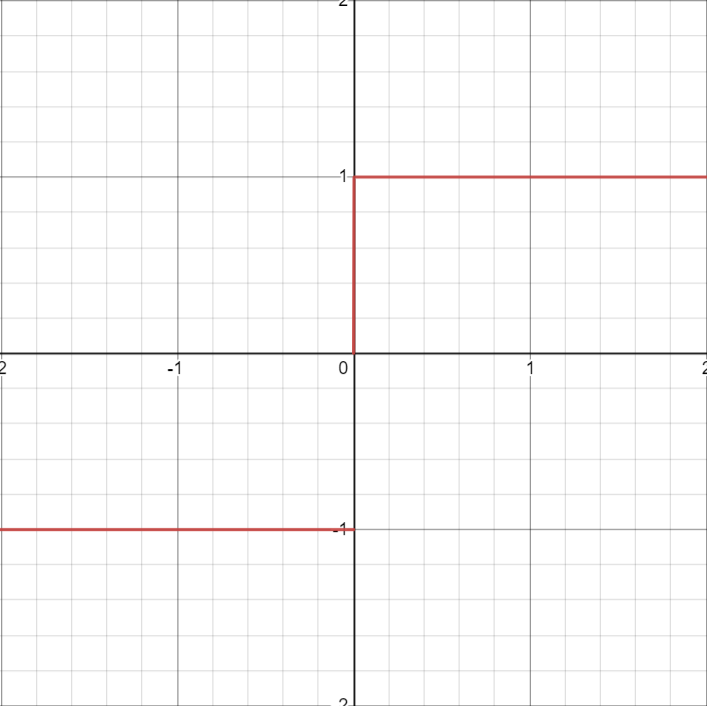
\includegraphics[scale=0.35]{11_1_2_1.png}
  
  \( \exists lim_{x \rightarrow 0} sign\ x \)

  \( lim_{x \rightarrow 0+} sign\ x = 1 \)

  \( lim_{x \rightarrow 0-} sign\ x = -1\)

  \( y = \frac{1}{x} \)

  \(lim_{x \rightarrow 0+0} \frac{1}{x} = +\infty\)

  \(lim_{x \rightarrow 0-0} \frac{1}{x} = -\infty\)
 \end{document}
